\documentclass[12pt,a4paper]{article}
\usepackage[utf8]{inputenc}
\usepackage[french]{babel}
\usepackage[T1]{fontenc}
\usepackage{amsmath}
\usepackage{inputenc}
\usepackage{amsfonts}
\usepackage{amssymb}
\usepackage{makeidx}
\usepackage{graphicx}
\usepackage[left=2cm,right=2cm,top=2cm,bottom=2cm]{geometry}
\author{Adrien Vigné}
\title{Outils Numériques Mécanique Rapport 1}
\begin{document}
\maketitle
\newpage
\tableofcontents
\newpage
\section{Activité 1 : Construction d'un système mécanique }
\subsection{Activité 1.1 : Créer une pièce dans le monde de la simulation}

\paragraph{Question :}
Description des différents blocs présents dans le modèle ouvert avec \textit{smnew}

\begin{figure}[h!]
\centering
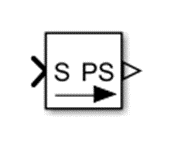
\includegraphics[width=.15\linewidth]{s_ps.png}
\caption{Permet de passer de la librairie simulink à la librairie simscape}
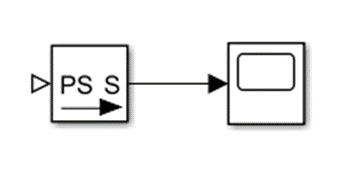
\includegraphics[width=.3\linewidth]{ps_s.png}
\caption{Permet de passer de la librairie simscape à la libraire simulink puis d’afficher le tracé des valeurs en fonction du temps ici}
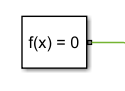
\includegraphics[width=.2\linewidth]{solveur.png}
\caption{Sert à paramétrer le solveur}
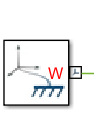
\includegraphics[width=.15\linewidth]{repere.png}
\caption{Représente le référentiel d’étude fixe}
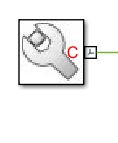
\includegraphics[width=.15\linewidth]{param.png}
\caption{Permet de fixer les paramètres mécaniques du modèle tel que la gravité}
\end{figure}
\begin{figure}[h!]
\centering
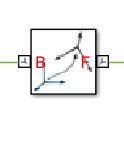
\includegraphics[width=.15\linewidth]{changement.png}
\caption{Représente un changement de base}
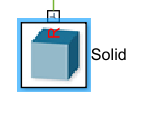
\includegraphics[width=.15\linewidth]{solid.png}
\caption{Représente un solide dans l’espace de modélisation}
\end{figure}
\newpage
\paragraph{Question : } Les positions des repères dans la modélisation.
Les repères mis en valeur sont ceux en surbrillance.

\begin{figure}[h!]
\centering 
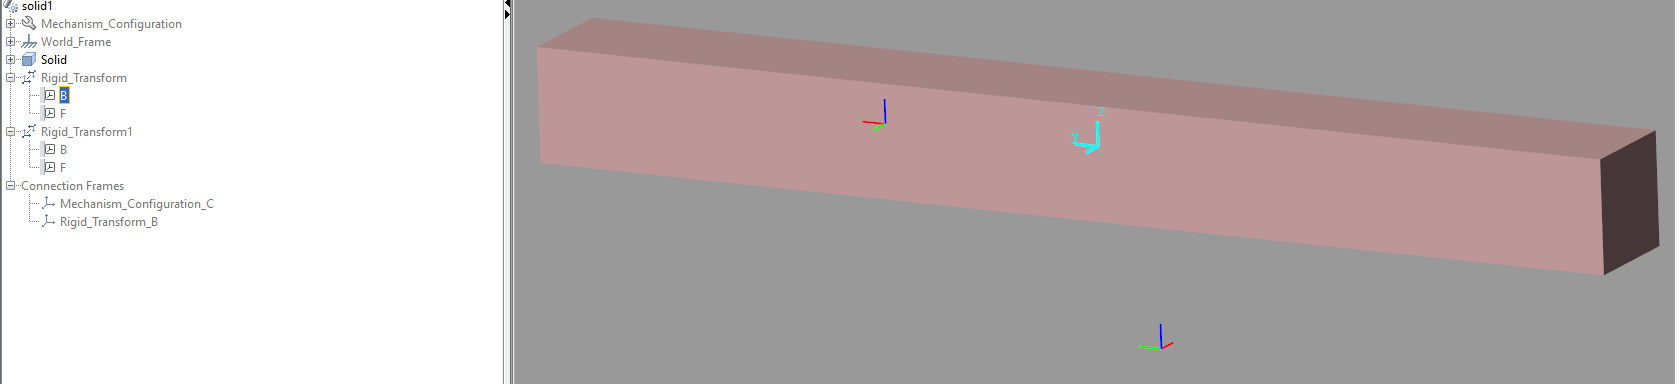
\includegraphics[width=.9\linewidth]{r1.png}
\caption{Repère d'entrée de la transformation 1}
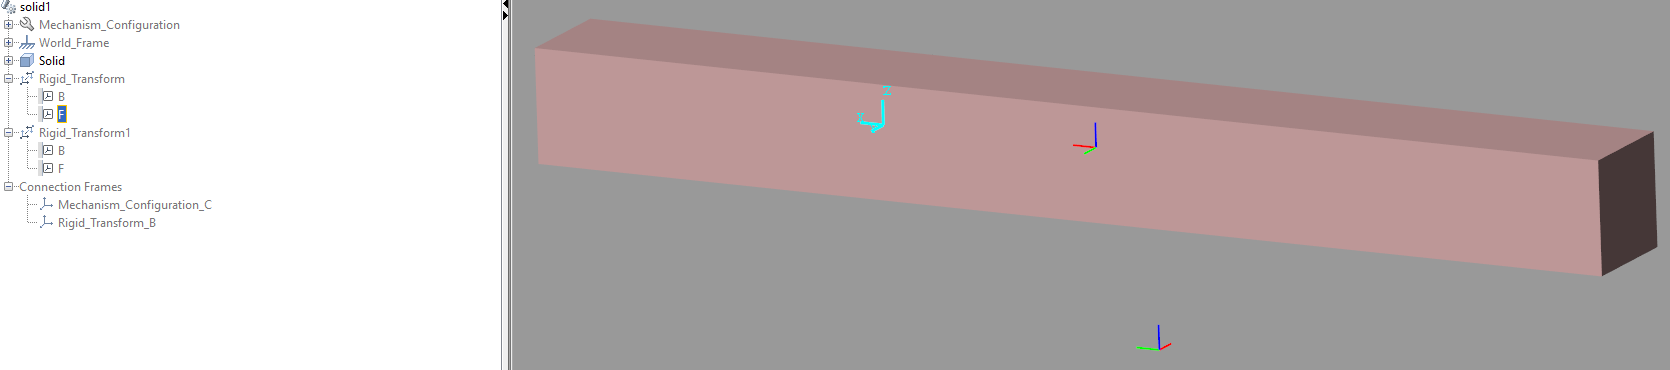
\includegraphics[width=.9\linewidth]{r2.png}
\caption{Repère de sortie de la transformation 1}
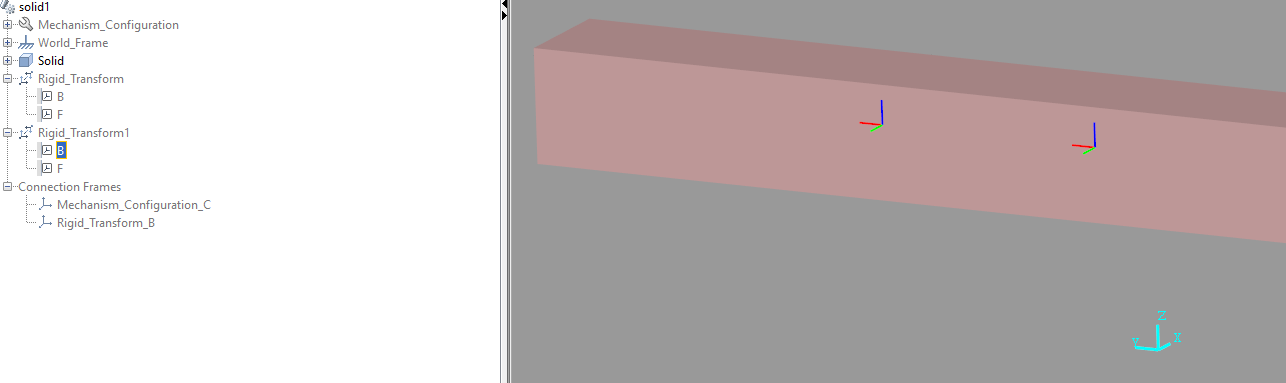
\includegraphics[width=.9\linewidth]{r3.png}
\caption{Repère d'entrée de la transformation 2}
\end{figure}
\newpage
Mise en place des repères de chaque coté du solide au centre des faces.
\begin{figure}[h!]
\centering
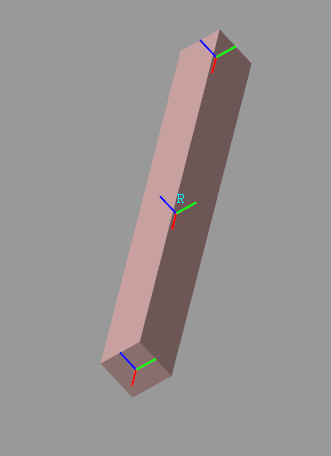
\includegraphics[scale=.9]{r4.png}
\caption{Pièce avec les repères placés comme voulu}
\end{figure}
\subsection{Activité 1.2 : Positionner une pièce par rapport à une autre}
En utilisant les blocs crées précédemment avec un angle de 45 deg entre la première pièce et la deuxième puis de 135 deg et un dernier de 45 deg.

\begin{figure}[h!]
\centering
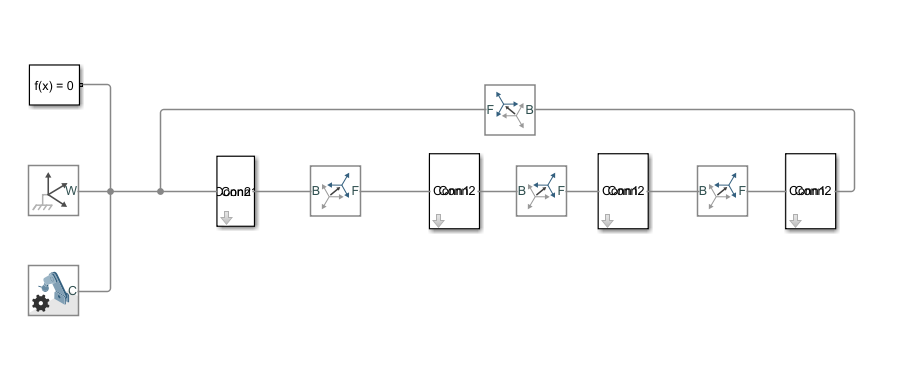
\includegraphics[width=.9\linewidth]{parallelo.png}
\caption{Modèle pour la construction du parallélogramme}
\end{figure}
\begin{figure}[h!]
\centering
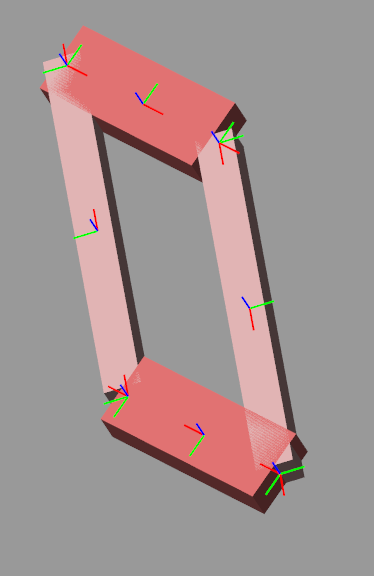
\includegraphics[scale=.9]{figure_paralallelo.png}
\caption{Parallélogramme modélisé}
\end{figure}
\newpage
\subsection{Activité 1.3 : Ajout d'un degré de liberté pouvant être actionné}
\paragraph{Question  : } Description des différents paramètres compris dans la liaison.
\begin{figure}[h!]
\centering
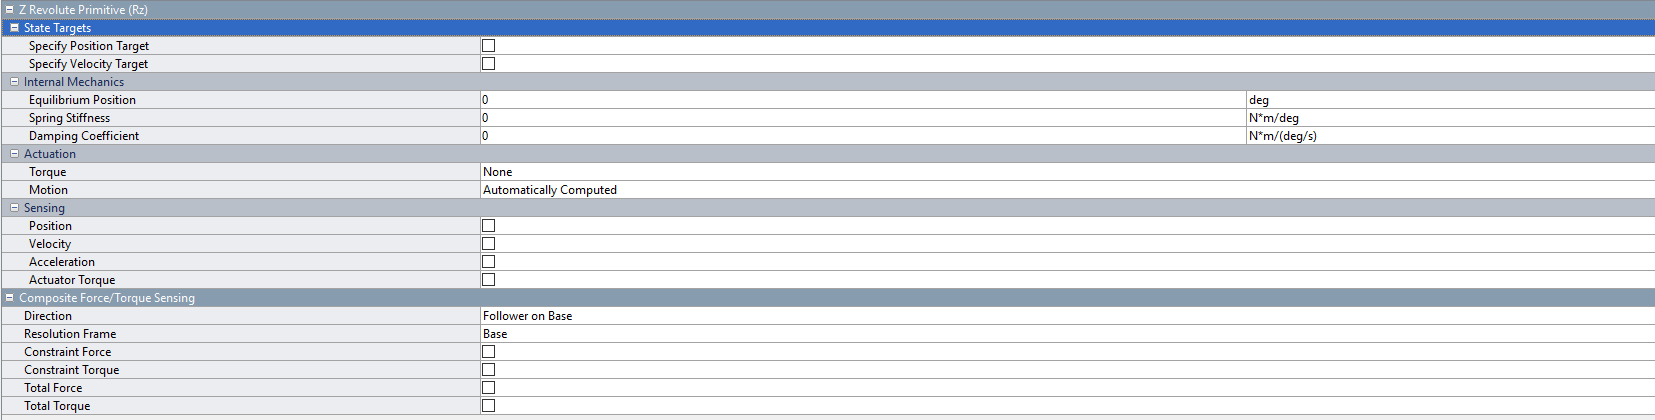
\includegraphics[width=.9\linewidth]{liaison.png}
\caption{Fenêtre de configuration de la liaison}
\end{figure}

\begin{description}
\item[State Target : ] permet de définir les positions initiales
\item[Internal Mechanics : ] permet de définir la raideur et les frottements dans la liaison
\item[Actuation : ] permet de définir si le couple et le mouvement sont calculés par la liaison ou définis par une entrée
\item[Sensing : ] permet d’activer des capteurs dans la liaison
\item[Composing Force/Torque Sensing : ] permet de récupérer les valeurs des efforts dans la liaison.
\end{description}

Motorisation d'une liaison.
\begin{figure}[h!]
\centering
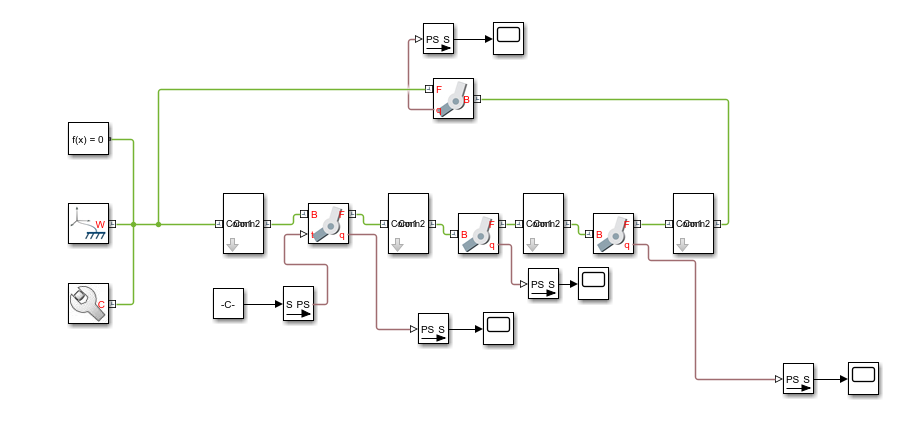
\includegraphics[width=.9\linewidth]{motorise.png}
\caption{Modèle du parallélogramme motorisé sur un angle}
\end{figure}

On remarque que l'une des grandes pièces est en translation circulaire par rapport à l'autre.
\section{Activité 2 : Modélisation de systèmes mécaniques simples}
\subsection{Activité 2.1 : Modélisation d’un système masse-ressort}
Hypothèse : Masse ponctuelle car on néglige les frottements sec devant l'effort du ressort et que la géométrie du solide n'intervient pas ici.

\begin{figure}[h!]
\centering
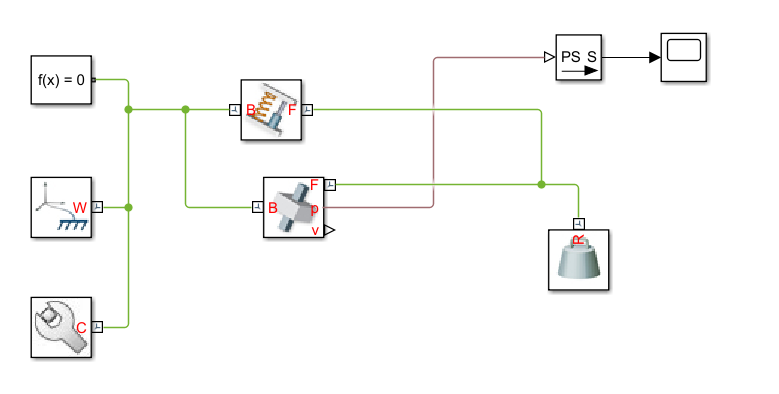
\includegraphics[width=.9\linewidth]{masse.png}
\caption{Modèle du système masse ressort}
\end{figure}

\paragraph{Mise en équation:}

\[ \ddot{x}+\dfrac{B}{m} \cdot \dot{x} + \dfrac{k}{m} \cdot x = \dfrac{k \cdot l_{0}}{m} \]
La solution de cette équation est : 
\[ x(t) = e^{-t/\tau} \cdot \left((x_{0}-l_{0}) \cdot \cos(\dfrac{\sqrt{\Delta}}{2}\cdot t)+ \dfrac{(x_{0}-l_{0}) B}{\sqrt{\Delta} m} \cdot \sin(\dfrac{\sqrt{\Delta}}{2}\cdot t) \right) + l_{0} \]

Avec \[\Delta = (\dfrac{B}{m})^2 - \dfrac{4 k}{m}\] et \[\tau = \dfrac{2 m }{B}\]
$x_0$ la longueur initiale, $l_0$ la longueur à vide du ressort 

En simulant on trouve : 

\begin{figure}[h!]
\centering
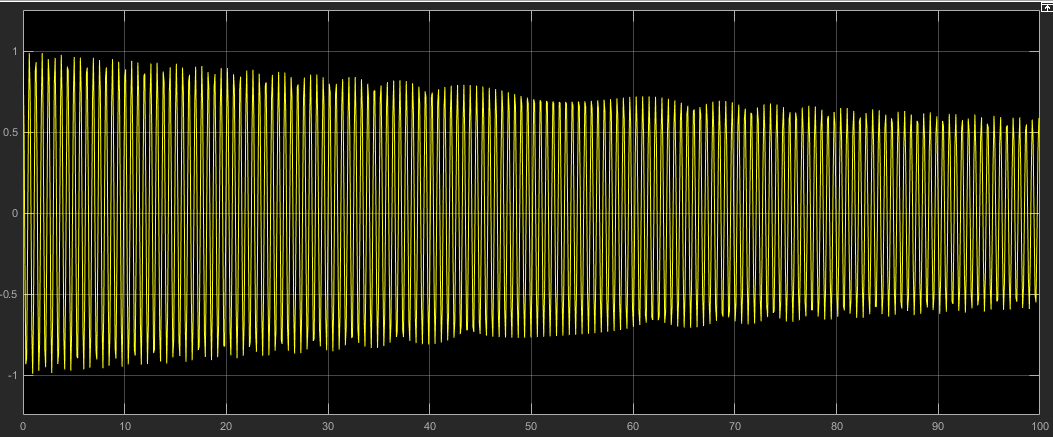
\includegraphics[width=.9\linewidth]{masse_resort.png}
\caption{Position de la masse avec le jeu de conditions initiales vitesse nul et $x=1$ m}
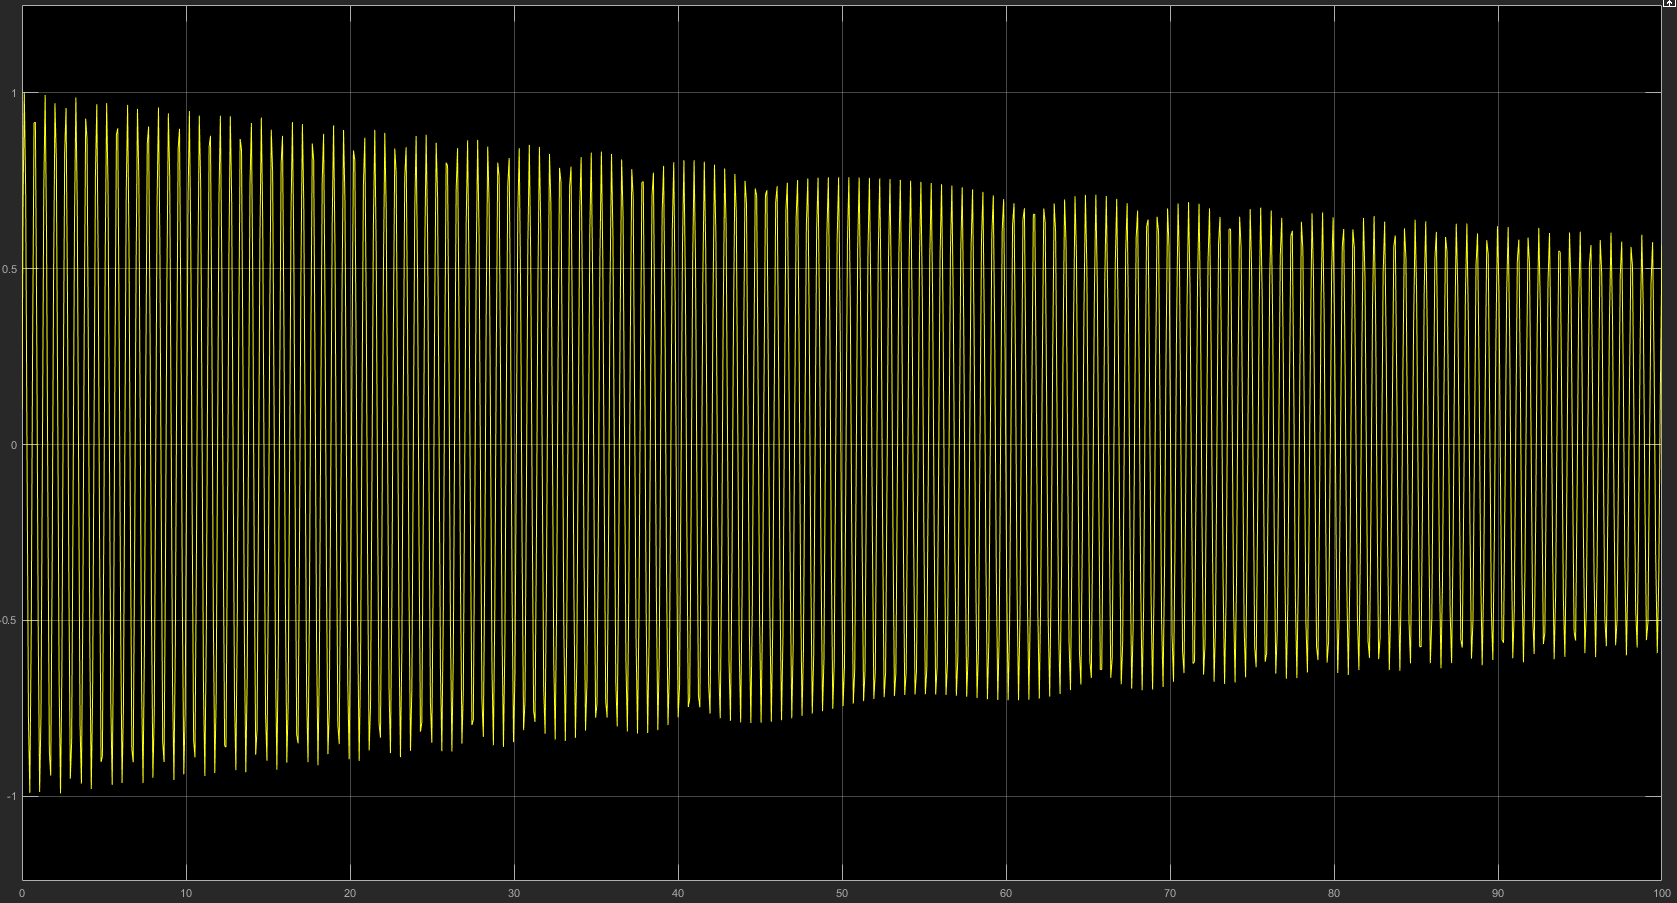
\includegraphics[width=.9\linewidth]{masse_resort2.png}
\caption{Position de la masse avec le jeu de conditions initiales $v=10$ m/s et $x=0.1$ m}
\end{figure}

Ce qui cohérent avec l'expression trouvé analytiquement.

\subsection{Activité 2.2 : Modélisation d'un pendule}
\paragraph{Mise en équation :} On néglige les frottements dans la liaison et les frottements visqueux. A partir de cela on en déduit en considérant comme force la gravité et la tension du fil, l'équation suivante :

\[ \ddot{\theta} + \dfrac{g}{l} \cdot \sin(\theta) = 0 \]

En faisant l'approximation des petits angles. On obtient l'équation :
\[ \ddot{\theta} + \dfrac{g}{l} \cdot \theta = 0 \]
Ce qui correspond au tracé obtenu en simulant sous MatLab. \\
\begin{figure}[h!]
\centering
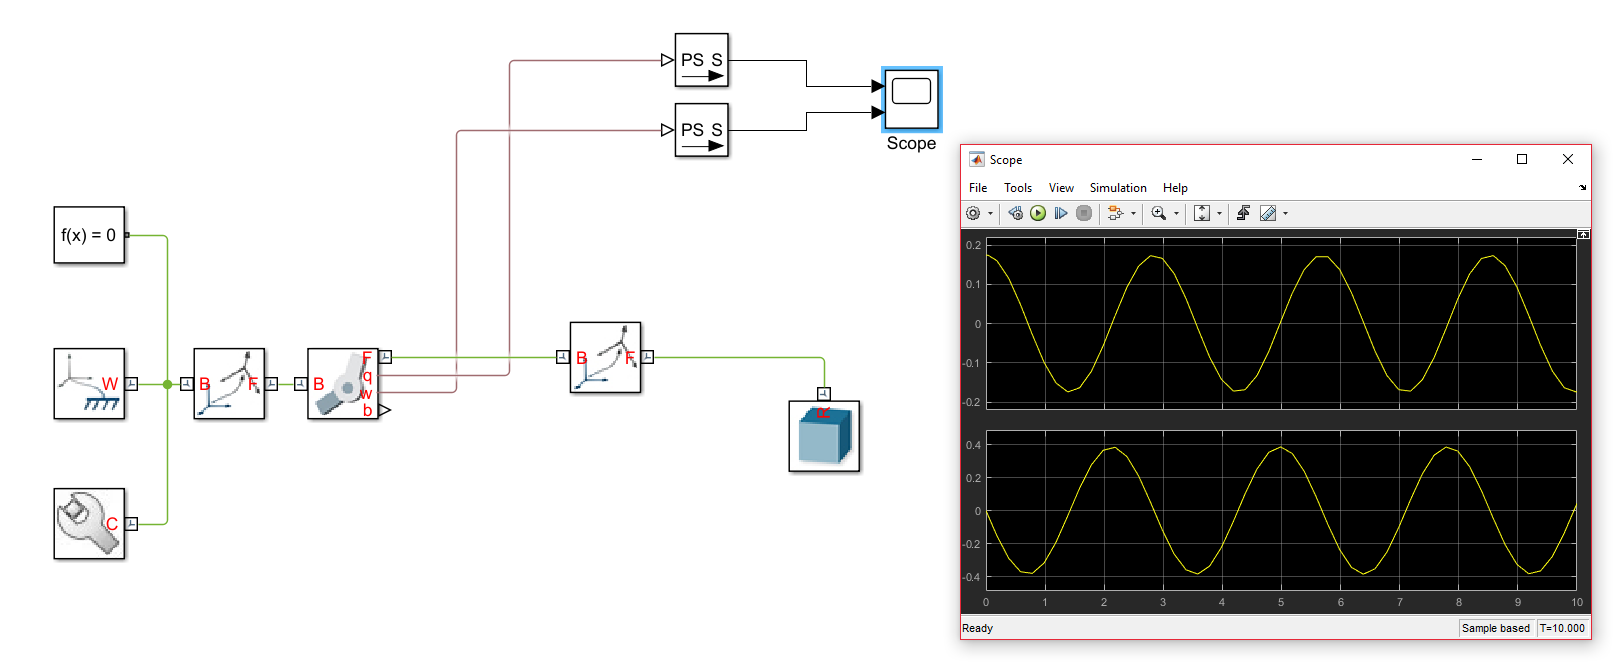
\includegraphics[width=.9\linewidth]{pendule1.png}
\caption{Modélisation du pendule et tracé de la positon et de la vitesse}
\end{figure}
\\
Dans le deuxième essai avec un angle de départ plus grand mais une corde plus courte on se retrouve dans des conditions identiques a l'approximation des petits angles.


\begin{figure}[h!]
\centering
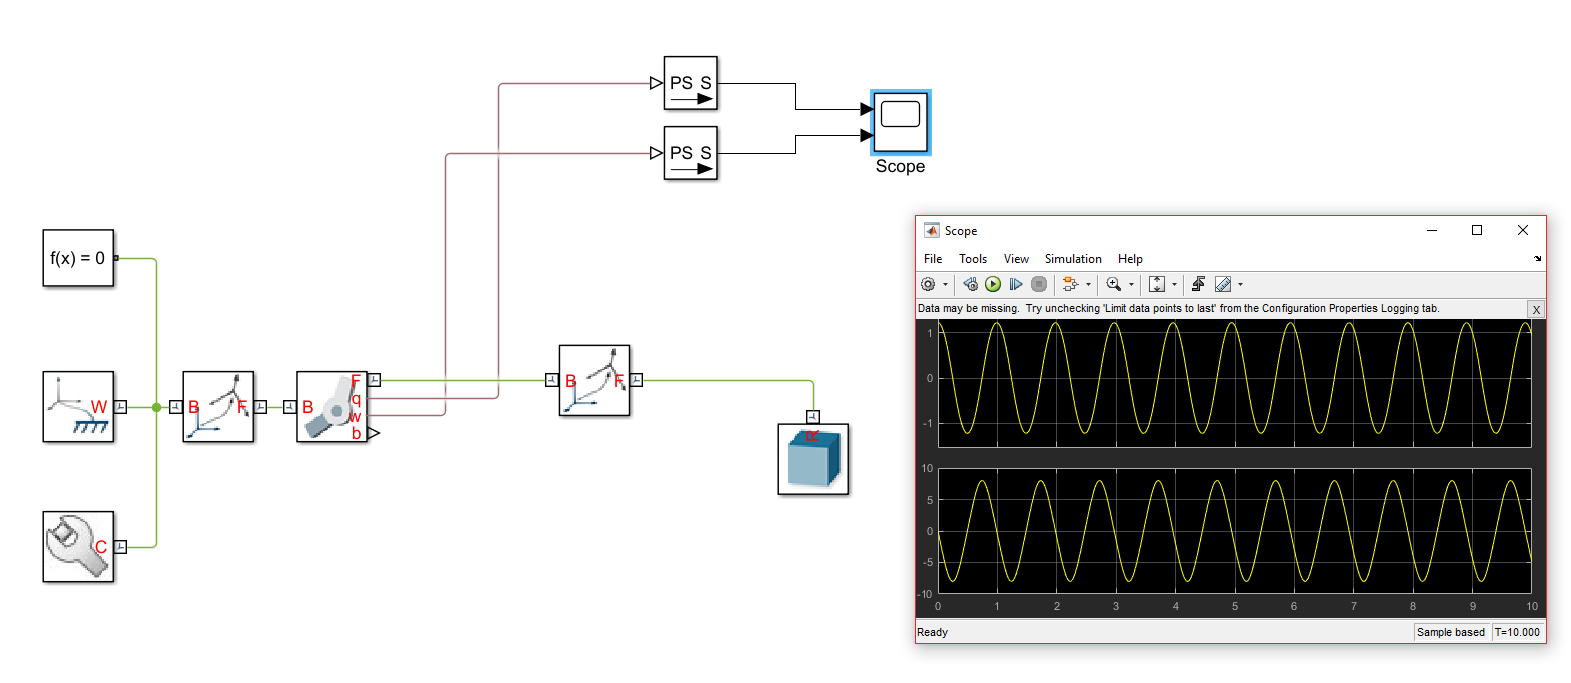
\includegraphics[width=.9\linewidth]{pendule2.png}
\caption{Modélisation du pendule et tracé de la positon et de la vitesse}
\end{figure}

\end{document}